\chapter{Architektura systemu}
\label{Chapter5}

\section{Wstęp}
\label{Chapter51}

System \textit{iQuest} został stworzony w oparciu o model architektury trójwarstwowej, w którym wyróżnione zostały warstwy: danych, logiki biznesowej oraz prezentacji. Dzięki takiemu podejściu, zadania związane z poszczególnymi warstwami można było bez większego problemu rozdzielić między członków zespołu programistów, a w przypadku ewentualnej modyfikacji jednej z warstw nie występuje konieczność wprowadzania zmian w reszcie projektu.

\section{Opis ogólny architektury -- ,,Marketektura''}
\label{Chapter52}

System \textit{iQuest} to aplikacja internetowa w postaci zbioru rozszerzeń platformy e-learningowej \textit{Moodle}. Całość (\textit{Moodle} oraz rozszrzenia) zainstalowana jest na serwerze www, zlokalizowanym w sieci Politechniki Poznańskiej, łączącym się z osobnym serwerem baz danych oraz usługami \textit{eKonto} i \textit{eDziekanat}. Funkcje raportowania realizowane są w głównej mierze za pośrednictwem zewnętrznego systemu \textit{BI}, pobierającego dane z \textit{iQuest} za pośrednictwem usług sieciowych (ang.~\definicja{webservices}). Administracja oraz obsługa systemu odbywa się za pośrednictwem przeglądarki internetowej, w ramach połączenia z platformą \textit{Moodle} lub serwerem raportowania. Respondenci mogą też uzyskać dostęp do systemu przy pomocy urządzeń mobilnych, takich jak tablety czy smartfony.

\begin{figure}[H]
\centering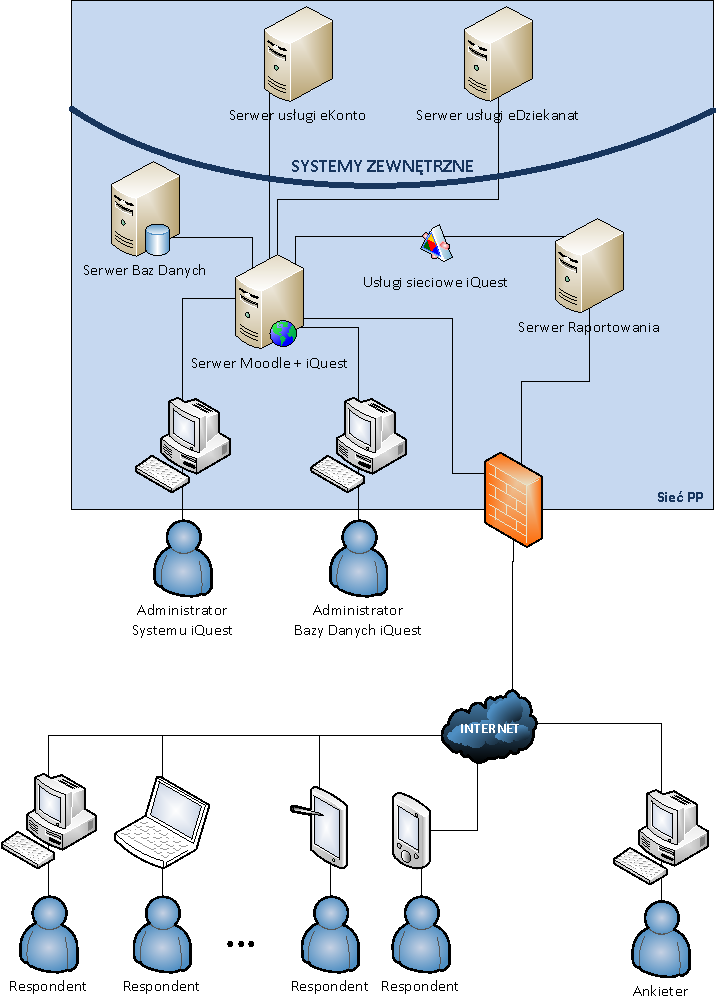
\includegraphics[width=0.9\textwidth]{figures/marketecture}
\caption{Diagram ,,Marketektury''}\label{rys:marketecture}
\end{figure}

\section{Analiza~podejść\slash Analiza~SWOT}
\label{Chapter53}

W fazie inicjacji projektu, zespół zarządzający przeprowadził analizę SWOT (ang. \definicja{Strengths, Weaknesses, Opportunities, Threats} - mocne strony, słabe strony, szanse, zagrożenia). Poniżej zamieszczono tabele \ref{tab:SWOT1}. oraz \ref{tab:SWOT2}., zawierające jej wyniki. W oparciu o nie, zespół zarządzający podjął decyzję o realizacji projektu z użyciem platformy \textit{Moodle}.

\begin{table}[H]
\centering
\begin{tabular}{ | p{2.5cm} | p{5.5cm} | p{5.5cm} | }
\hline
--- & \textbf{Pozytywne} & \textbf{Negatywne} \\ \hline
\multirow{6}{*}{\textbf{Wewnętrzne}} & \textbf{Mocne strony (S)} & \textbf{Słabe strony (W)} \\
			& Środowisko \textit{Moodle} jest dobrze udokumentowane\cite{Man:Moodle}. & Konieczność trzymania się standardów \textit{Moodle}. \\
			& Środowisko \textit{Moodle} jest łatwe w rozwoju. & Konieczność wdrożenia się w nieznany kod. \\
			& Stosowanie podejścia MVC w środowisku \textit{Moodle}. & \\
			& Już zaimplementowane mechanizmy, takie jak kontrola praw dostępu, CMS. & \\
			& Posiadanie bazy wiedzy, która ma zachęcać użytkowników. & \\ \hline
%					
\multirow{3}{*}{\textbf{Zewnętrzne}} & \textbf{Szanse (O)} & \textbf{Zagrożenia (T)} \\
				& Modułowość platformy \textit{Moodle}. & Środowisko może być nieznane programistom. \\
				& Łatwość tworzenia własnych wtyczek. & \\ \hline
\end{tabular}
\caption{Podejście pierwsze -- w oparciu o platformę \textit{Moodle}}\label{tab:SWOT1}
\end{table}

\begin{table}[H]
\centering
\begin{tabular}{ | p{2.5cm} | p{5.5cm} | p{5.5cm} | }
\hline
--- & \textbf{Pozytywne} & \textbf{Negatywne} \\ \hline
\multirow{2}{*}{\textbf{Wewnętrzne}} & \textbf{Mocne strony (S)} & \textbf{Słabe strony (W)} \\
			& Dostępność platformy na wszystkich popularnych systemach operacyjnych. & Konieczność implementacji dodatkowych funkcjonalności związanych z zachęcaniem do korzystania z systemu. \\ \hline
%					
\multirow{3}{*}{\textbf{Zewnętrzne}} & \textbf{Szanse (O)} & \textbf{Zagrożenia (T)} \\
				& Dobra znajomość kodu przez programistów. & Konieczność tworzenia wszystkiego od podstaw. \\
				& & Nieznajomość technologii przez programistów. \\ \hline
\end{tabular}
\caption{Podejście drugie -- napisanie aplikacji od podstaw przy użyciu \textit{Java~EE}}\label{tab:SWOT2}
\end{table}

Rozpatrując powyższe tabele z perspektywy czasu, autorzy niniejszej pracy stwierdzili, iż analiza SWOT została zrealizowana nieprawidłowo, faworyzując rozwiązanie z użyciem systemu \textit{Moodle}. Dla przykładu, dokumentacja \textit{Moodle} okazała się być w znacznym stopniu nieprecyzyjna i niekompletna, zaś w kodzie platformy nie stosuje się podejścia MVC.

\section{Perspektywy architektoniczne}
\label{Chapter54}

\subsection{Perspektywa fizyczna}
\label{Chapter541}

\begin{figure}[H]
\centering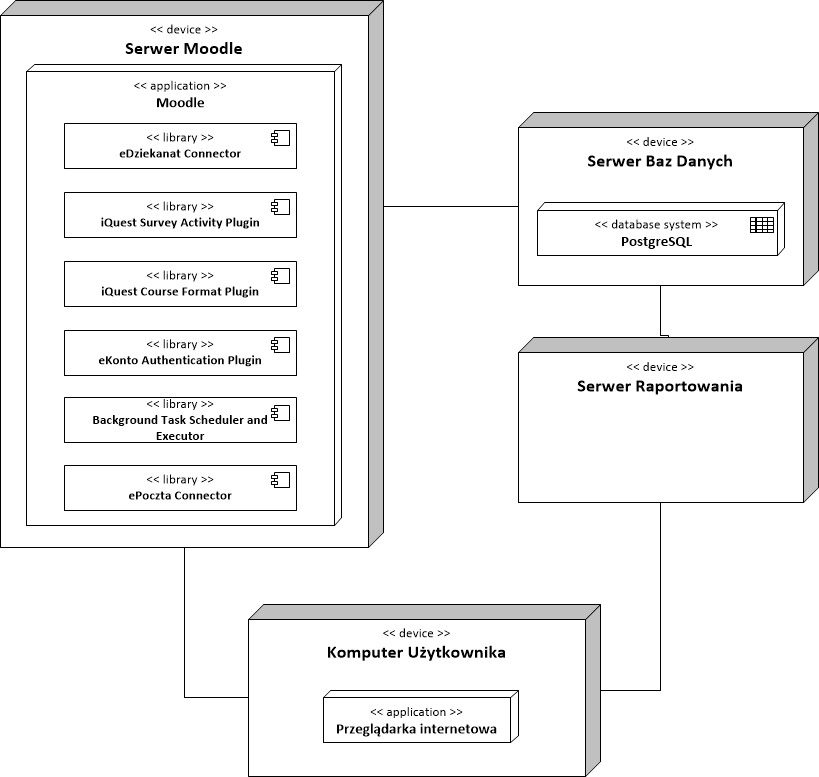
\includegraphics[width=0.9\textwidth]{figures/PhysicalView}
\caption{Diagram perspektywy fizycznej}\label{rys:PerspektywaFizyczna}
\end{figure}

Schemat \ref{rys:PerspektywaFizyczna} prezentuje perspektywę fizyczną projektu. Widać na nim dokładnie, opisaną wcześniej, opartą na rozszerzeniach dla platformy \textit{Moodle} budowę logiki systemu \textit{iQuest}. Za jej pośrednictwem dokonuje się połączeń z serwerem baz danych oraz serwerem raportowania. Użytkownik systemu, z wykorzystaniem przeglądarki internetowej, komunikuje się z platformą, lub systemem raportowania, korzystając przy tym z warstwy prezentacji.

\subsection{Perspektywa logiczna}
\label{Chapter542}

\begin{figure}[H]
\centering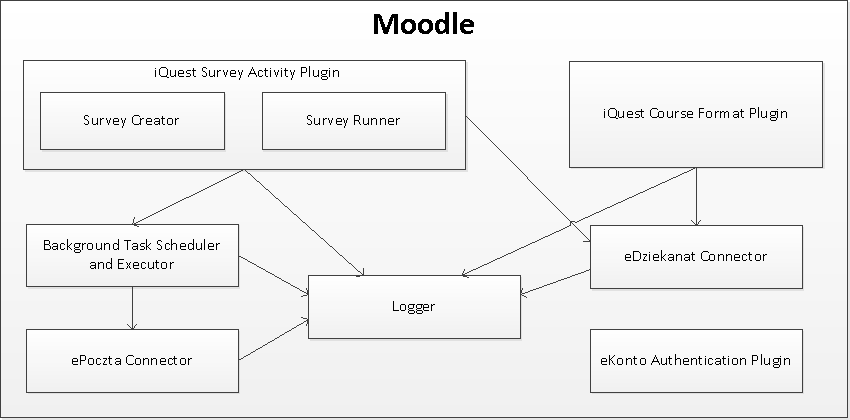
\includegraphics[width=0.9\textwidth]{figures/LogicalView}
\caption{Diagram perspektywy logicznej}\label{rys:PerspektywaLogiczna}
\end{figure}

Schemat \ref{rys:PerspektywaLogiczna} prezentuje perspektywę logiczną systemu. Określa ona zależności między poszczególnymi komponentami ,,wszczepionymi'' do platformy \textit{Moodle}. Poniżej znajduje się opis wyszczególnionych na rysunku komponentów.

\subsubsection{iQuest Survey Activity Plugin}
\label{Chapter5421}
Funkcjonalnością \definicja{Activity Plugin} jest udostępnianie możliwości dodania nowych rodzajów tzw. ,,aktywności'' w ramach platformy \textit{Moodle}. \textit{iQuest Survey Activity Plugin} pozwala na dodanie nowego badania \textit{iQuest}. Komponent ten składa się z dwóch subkomponentów:
\begin{itemize}
\item{Survey Creator}
\item{Survey Runner}
\end{itemize}
Pierwszy z nich odpowiada za definiowanie ankiet, natomiast drugi za ich realizację.

\subsubsection{iQuest Course Format Plugin}
\label{Chapter5422}

\definicja{Course Format Plugin} dla platformy \textit{Moodle} odpowiada za obsługę interfejsu użytkownika. W przypadku systemu \textit{iQuest}, zarządza kwestią wyświetlania użytkownikowi tylko tych składowych kursu związanego z systemem \textit{iQuest}, które są dla niego dostępne. Przykładowo, Respondent uzyska dostęp do listy ankiet, które może wypełnić, podczas gdy ankieter uzyska dostęp do listy zarządzanych przez niego badań.

\subsubsection{eDziekanat Connector oraz ePoczta Connector}
\label{Chapter5423}

Komponenty te odpowiadają za komunikację z usługami \textit{eDziekanat} i \textit{ePoczta}, pozwalające m.in. na pozyskanie danych o grupach docelowych (w oparciu o dane Grup Dziekańskich) oraz wysyłanie powiadomień za pośrednictwem poczty studenckiej.

\subsubsection{Background Task Scheduler and Executor}
\label{Chapter5424}

Dzięki temu komponentowi możliwe jest szeregowanie oraz wykonywanie zadań w tle. Jednym z jego zadań jest kolejkowanie i aktywowanie mechanizmów rozsyłania wiadomości e-mail z zaproszeniami do udziału w ankiecie.

\subsubsection{eKonto Authentication Plugin}
\label{Chapter5425}

\definicja{eKonto Authentication Plugin} -- to moduł uwierzytelniania (ang.~\definicja{Authentication}), korzystający z systemu \textit{eLogin} platformy \textit{eKonto} do logowania się do platformy \textit{Moodle}, obsługującej system \textit{iQuest}. Korzystanie z tego systemu pozwala nie tylko na jednoznaczną weryfikację tożsamości użytkownika łączącego się z systemem, ale jest zarazem wygodne -- dzięki jego zastosowaniu, nie ma potrzeby posiadania osobnego konta w systemie \textit{iQuest}.

\subsection{Perspektywa implemetancyjna}
\label{Chapter543}

\begin{figure}[H]
\centering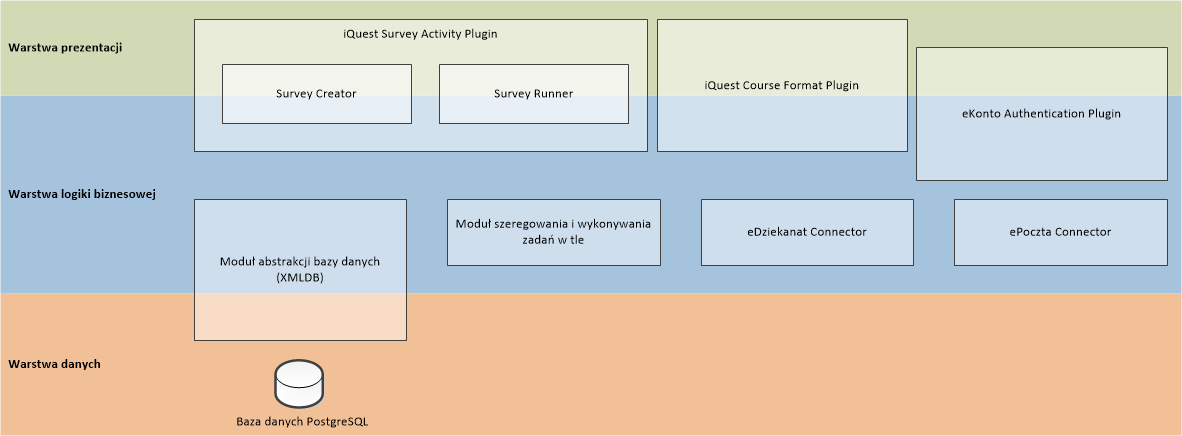
\includegraphics[width=0.9\textwidth]{figures/Layers}
\caption{Diagram perspektywy implementacyjnej}\label{rys:PerspektywaImplementacyjna}
\end{figure}

Diagram perspektywy implementacyjnej (rys.~\ref{rys:PerspektywaImplementacyjna}) pozwala na analizę przeplatania się elementów systemu \textit{iQuest} w ramach poszczególnych warstw zastosowanego modelu trójwarstwowego. Funkcje zaprezentowanych na nim modułów zostały wyjaśnione już wcześniej w niniejszym dokumencie.

\section{Decyzje projektowe}
\label{Chapter55}

\subsection{Wstęp}
\label{Chapter551}

W procesie rozwoju systemu \textit{iQuest} podjęto dokładnie 40 decyzji projektowych. Większość decyzji podejmował Architekt. W części przypadków rozpatrywano także zdanie zespołu programistów.

\subsection{Podjęte decyzje}
\label{Chapter552}

%1
\begin{table}[H]
\centering
\begin{tabular}{ | >{\bfseries}c | p{11cm} | }
\hline
%
Identyfikator & D01 \\ \hline
Nazwa & Postać systemu \\ \hline
Opis & System iQuest jest zestawem rozszerzeń środowiska \textit{Moodle} \\ \hline
Uzasadnienie & Platforma \textit{Moodle} jest już stosowana na uczelni, więc łatwiej jest dotrzeć z ankietami do studentów, jeżeli można je wypełniać bezpośrednio w \textit{Moodle'u}. \\ \hline
Źródło & Architekt \\ \hline
%
\end{tabular}
\end{table}

%2
\begin{table}[H]
\centering
\begin{tabular}{ | >{\bfseries}c | p{11cm} | }
\hline
%
Identyfikator & D02 \\ \hline
Nazwa & Podział na komponenty  \\ \hline
Opis & \textit{iQuest} składa się z następujących głównych komponentów: \textit{iQuest Course Format Plugin}, \textit{iQuest Survey Activity Plugin}, \textit{eDziekanat Connector}, \textit{eKonto Authentication Plugin}, \textit{Background Task Scheduler and Executor}, \textit{Logger}  \\ \hline
Uzasadnienie & Dzięki budowie modułowej łatwiej jest analizować, implementować i testować system. \\ \hline
Źródło & Architekt \\ \hline
%
\end{tabular}
\end{table}

%3
\begin{table}[H]
\centering
\begin{tabular}{ | >{\bfseries}c | p{11cm} | }
\hline
%
Identyfikator & D03 \\ \hline
Nazwa & \textit{iQuest} jako kurs na \textit{Moodle'u}  \\ \hline
Opis & \textit{iQuest} widoczny jest dla użytkowników platformy \textit{Moodle} jako specjalny kurs. \\ \hline
Uzasadnienie & Jest to zgodne z ideą \textit{Moodle'a} -- treści umieszczane na tej platformie są pogrupowane w kursach. \\ \hline
Źródło & Architekt \\ \hline
%
\end{tabular}
\end{table}

%4
\begin{table}[H]
\centering
\begin{tabular}{ | >{\bfseries}c | p{11cm} | }
\hline
%
Identyfikator & D04 \\ \hline
Nazwa & Wtyczka \textit{iQuest Course Format Plugin}  \\ \hline
Opis & \textit{iQuest Course Format Plugin} odpowiada za prezentowanie treści wewnątrz kursu, w ramach którego funkcjonuje system \textit{iQuest}. Plugin dba o to, aby ankieterowi wyświetlała się lista tylko tych badań, do których ma on uprawnienia oraz żeby respondent widział listę tylko tych badań, w których ma on prawo wypełnić ankietę. \\ \hline
Uzasadnienie & Istnienie takiej wtyczki jest wymagane, ponieważ bez niej nie byłoby możliwe filtrowanie listy badań tak, aby użytkownik wydział tylko te do których ma uprawnienia. \\ \hline
Źródło & Architekt \\ \hline
%
\end{tabular}
\end{table}

%5
\begin{table}[H]
\centering
\begin{tabular}{ | >{\bfseries}c | p{11cm} | }
\hline
%
Identyfikator & D05 \\ \hline
Nazwa & \textit{Wtyczka eKonto Authentication Plugin}  \\ \hline
Opis & Logowanie użytkowników przy pomocy \textit{eKonta} realizowane jest poprzez utworzenie rozszerzenia \textit{eKonto Authentication Plugin} dla platformy \textit{Moodle}. \\ \hline
Uzasadnienie & Platforma \textit{Moodle} jest tak skonstruowana, że aby umożliwić uwierzytelnianie przy pomocy zewnętrznych mechanizmów, konieczne jest utworzenie specjalnej wtyczki. \\ \hline
Źródło & Architekt \\ \hline
%
\end{tabular}
\end{table}

%6
\begin{table}[H]
\centering
\begin{tabular}{ | >{\bfseries}c | p{11cm} | }
\hline
%
Identyfikator & D06 \\ \hline
Nazwa & Wtyczka \textit{iQuest Survey Activity Plugin} - funkcjonalność dla ankieterów  \\ \hline
Opis & \textit{iQuest Survey Activity Plugin} pozwala ankieterowi na tworzenie, edytowanie i usuwanie ankiet, a także na tworzenie, edytowanie i usuwanie badań. \\ \hline
Uzasadnienie & Wtyczka typu \textit{Activity Plugin} dla \textit{Moodle'a} posiada wszystkie cechy potrzebne do zrealizowania tego typu funkcjonalności w sposób intuicyjny dla użytkownika. \\ \hline
Źródło & Architekt \\ \hline
%
\end{tabular}
\end{table}

%7
\begin{table}[H]
\centering
\begin{tabular}{ | >{\bfseries}c | p{11cm} | }
\hline
%
Identyfikator & D07 \\ \hline
Nazwa & Wtyczka \textit{iQuest Survey Activity Plugin} - funkcjonalność dla respondentów \\ \hline
Opis & \textit{iQuest Survey Activity Plugin} pozwala respondentowi na udzielenie odpowiedzi w ankiecie. \\ \hline
Uzasadnienie & Wtyczka typu \textit{Activity Plugin} dla \textit{Moodle'a} posiada wszystkie cechy potrzebne do zrealizowania tego typu funkcjonalności w sposób intuicyjny dla użytkownika. \\ \hline
Źródło & Architekt \\ \hline
%
\end{tabular}
\end{table}

%8
\begin{table}[H]
\centering
\begin{tabular}{ | >{\bfseries}c | p{11cm} | }
\hline
%
Identyfikator & D08 \\ \hline
Nazwa & Wykorzystanie protokołu HTTPS \\ \hline
Opis & \textit{Moodle} (w ramach którego działa \textit{iQuest}) będzie dostępny dla użytkowników poprzez protokół HTTPS. \\ \hline
Uzasadnienie & Zastosowanie protokołu HTTPS jest łatwym sposobem na dość skuteczne zabezpieczenie danych przesyłanych między klientem a serwerem. \\ \hline
Źródło & Architekt \\ \hline
%
\end{tabular}
\end{table}

%9
\begin{table}[H]
\centering
\begin{tabular}{ | >{\bfseries}c | p{11cm} | }
\hline
%
Identyfikator & D09 \\ \hline
Nazwa & Mechanizm kont i ról użytkowników \\ \hline
Opis & Wykorzystany jest istniejący w systemie \textit{Moodle} mechanizm kont i ról użytkowników. \\ \hline
Uzasadnienie & Dzięki temu nie ma potrzeby implementowania osobnego mechanizmu. Ten istniejący w \textit{Moodle'u} spełnia niezbędne wymagania. \\ \hline
Źródło & Architekt \\ \hline
%
\end{tabular}
\end{table}

%10
\begin{table}[H]
\centering
\begin{tabular}{ | >{\bfseries}c | p{11cm} | }
\hline
%
Identyfikator & D10 \\ \hline
Nazwa & Integracja \textit{eKonta} z kontem na \textit{Moodle'u} \\ \hline
Opis & W momencie pierwszego logowania danego użytkownika przy pomocy \textit{eKonta}, jest mu tworzone profil w systemie \textit{Moodle}. Za nazwę użytkownika przyjmuje się adres e-mail. Do profilu, dzięki możliwościom usługi \textit{eKonto} kopiowane są także inne dane użytkownika (np. imię i nazwisko). \\ \hline
Uzasadnienie & Takie działanie jest wymagane, aby zainicjalizować konto użytkownika logującego się do \textit{Moodle'a} przez \textit{eKonto} po raz pierwszy. \\ \hline
Źródło & Architekt \\ \hline
%
\end{tabular}
\end{table}

%11
\begin{table}[H]
\centering
\begin{tabular}{ | >{\bfseries}c | p{11cm} | }
\hline
%
Identyfikator & D11 \\ \hline
Nazwa & Sposób zapamiętywania ustawień systemu \textit{iQuest}  \\ \hline
Opis & Ustawienia systemu \textit{iQuest} przechowywane są w specjalnej tabeli bazy danych, w postaci identyfikator-wartość, które są ciągami znaków. \\ \hline
Uzasadnienie & Umożliwia to łatwy i wygodny dostęp do ustawień w różnych miejscach kodu źródłowego systemu. \\ \hline
Źródło & Architekt \\ \hline
%
\end{tabular}
\end{table}

%12
\begin{table}[H]
\centering
\begin{tabular}{ | >{\bfseries}c | p{11cm} | }
\hline
%
Identyfikator & D12 \\ \hline
Nazwa & Dziennik zdarzeń \\ \hline
Opis & Wszystkie ważniejsze zdarzenia w systemie \textit{iQuest} są zapisywane w logu w bazie danych, w specjalnej tabeli. Dla każdego zdarzenia zapisane zostaną następujące dane: data i godzina, identyfikator użytkownika wykonującego operację (o ile dotyczy), tekstowy opis, typ (informacja, ostrzeżenie, błąd). \\ \hline
Uzasadnienie & Mechanizm logowania zdarzeń obecny w \textit{Moodle'u} nie spełnia wymagań - nie pozwala na dzielenie wpisów na kategorie. Z tego powodu została podjęta decyzja o utworzeniu osobnego mechanizmu. \\ \hline
Źródło & Architekt \\ \hline
%
\end{tabular}
\end{table}

%13
\begin{table}[H]
\centering
\begin{tabular}{ | >{\bfseries}c | p{11cm} | }
\hline
%
Identyfikator & D13 \\ \hline
Nazwa & Listy ACL dla badań \\ \hline
Opis & Z każdą ankietą jest powiązana lista ACL zawierająca informacje o tym, którzy użytkownicy mają prawo wykorzystywać ankietę w swoim badaniu, którzy mogą ją edytować, a którzy mogą ją usuwać. \\ \hline
Uzasadnienie & Jest to elastyczny sposób zarządzania uprawnieniami do ankiet. \\ \hline
Źródło & Architekt \\ \hline
%
\end{tabular}
\end{table}

%14
\begin{table}[H]
\centering
\begin{tabular}{ | >{\bfseries}c | p{11cm} | }
\hline
%
Identyfikator & D14 \\ \hline
Nazwa & Wpisy na listach ACL dla badań - rodzaje podmiotów \\ \hline
Opis & Wpisy na listach ACL wspomnianych w decyzji D13 mogą dotyczyć konkretnych użytkowników, albo ról. \\ \hline
Uzasadnienie & Znacznie ułatwi to zarządzanie uprawnieniami do ankiet. \\ \hline
Źródło & Architekt \\ \hline
%
\end{tabular}
\end{table}

%15
\begin{table}[H]
\centering
\begin{tabular}{ | >{\bfseries}c | p{11cm} | }
\hline
%
Identyfikator & D15 \\ \hline
Nazwa & Wykonywanie zadań w tle \\ \hline
Opis & System \textit{iQuest} posiada możliwość wykonywania złożonych zadań w tle. Poszczególne moduły systemu mogą dodawać zlecenia, z których każde składa się z jednego lub wielu zadań. \\ \hline
Uzasadnienie & Pozwala to na poprawienie responsywności systemu dla użytkownika (np. ankieter nie musi czekać, aż wyślą się e-maile z zaproszeniami dla respondentów). Podział zleceń na zadania umożliwia łatwiejszą obsługę sytuacji, w której w trakcie realizowania zlecenia następuje awaria - zadania już wykonane nie zostaną wykonane ponownie, a wykonane zostaną tylko zadania niewykonane wcześniej. \\ \hline
Źródło & Architekt \\ \hline
%
\end{tabular}
\end{table}

%16
\begin{table}[H]
\centering
\begin{tabular}{ | >{\bfseries}c | p{11cm} | }
\hline
%
Identyfikator & D16 \\ \hline
Nazwa & Kolejkowanie zadań wykonywanych w tle \\ \hline
Opis & Moduł wykonywana zadań w tle posiada mechanizm kolejkowania. \\ \hline
Uzasadnienie & Pozwala to na zwiększenie niezawodności systemu (np. e-maile do wysłania nie "przepadną" a zostaną zakolejkowane w przypadku awarii \textit{ePoczty}). \\ \hline
Źródło & Architekt \\ \hline
%
\end{tabular}
\end{table}

%17
\begin{table}[H]
\centering
\begin{tabular}{ | >{\bfseries}c | p{11cm} | }
\hline
%
Identyfikator & D17 \\ \hline
Nazwa & Priorytety zadań kolejkowanych do wykonania w tle \\ \hline
Opis & Zlecenia do wykonania w tle posiadają priorytety. Mechanizm kolejkowania w pierwszej kolejności wybiera do wykonania zlecenia o najwyższym priorytecie. \\ \hline
Uzasadnienie & Pozwala to na wykonanie najważniejszych zadań w pierwszej kolejności. \\ \hline
Źródło & Architekt \\ \hline
%
\end{tabular}
\end{table}

%18
\begin{table}[H]
\centering
\begin{tabular}{ | >{\bfseries}c | p{11cm} | }
\hline
%
Identyfikator & D18 \\ \hline
Nazwa & Identyfikowanie modułów mających wykonać zadanie w tle \\ \hline
Opis &  	Każde zadanie do wykonania w tle posiada identyfikator modułu, jaki powinien je wykonać. \\ \hline
Uzasadnienie & Zadania do wykonania w tle mają różne rodzaje. Umożliwi to systemowi w łatwy sposób uruchomić kod odpowiedni do wykonania danego rodzaju zadania. \\ \hline
Źródło & Architekt \\ \hline
%
\end{tabular}
\end{table}

%19
\begin{table}[H]
\centering
\begin{tabular}{ | >{\bfseries}c | p{11cm} | }
\hline
%
Identyfikator & D19 \\ \hline
Nazwa &  Sposób przechowywania danych niezbędnych do wykonania zadania w tle \\ \hline
Opis & Dane niezbędne do wykonania zadania przechowywane są w odpowiedniej kolumnie bazy danych w postaci łańcucha znakowego. Dane te mają postać obiektu zserializowanego przy pomocy technologii \textit{JSON}. \\ \hline
Uzasadnienie & Zadania do wykonania w tle mają różne rodzaje. Umożliwi to systemowi w łatwy sposób uruchomić kod odpowiedni do wykonania danego rodzaju zadania. \\ \hline
Źródło & Architekt \\ \hline
%
\end{tabular}
\end{table}

%20
\begin{table}[H]
\centering
\begin{tabular}{ | >{\bfseries}c | p{11cm} | }
\hline
%
Identyfikator & D20 \\ \hline
Nazwa & Zewnętrzny system \textit{BI} \\ \hline
Opis & Do generowania raportów wykorzystany jest system \textit{BI} działający na osobnym serwerze. \\ \hline
Uzasadnienie & Dzięki temu nie trzeba implementować od początku mechanizmu raportowania, a można wykorzystać istniejące już oprogramowanie.  \\ \hline
Źródło & Architekt \\ \hline
%
\end{tabular}
\end{table}

%21
\begin{table}[H]
\centering
\begin{tabular}{ | >{\bfseries}c | p{11cm} | }
\hline
%
Identyfikator & D21 \\ \hline
Nazwa & Wykonywanie zadań przez osobny proces \\ \hline
Opis & Po dodaniu zlecenia do wykonania w tle, na serwerze uruchamiany jest proces wykonujący zadania. \\ \hline
Uzasadnienie & Umożliwia to natychmiastowe rozpoczęcie wykonywania zadań. Utworzenie procesu pozwoli na przetwarzanie w tle. \\ \hline
Źródło & Architekt \\ \hline
%
\end{tabular}
\end{table}

%22
\begin{table}[H]
\centering
\begin{tabular}{ | >{\bfseries}c | p{11cm} | }
\hline
%
Identyfikator & D22 \\ \hline
Nazwa & Maksymalnie 1 proces wykonujący przetwarzanie w tle \\ \hline
Opis &  	Zadania w tle wykonywane są przez 1 proces na serwerze. \\ \hline
Uzasadnienie & Ułatwia to implementację - można uniknąć problemów związanych ze współbieżnością. \\ \hline
Źródło & Architekt \\ \hline
%
\end{tabular}
\end{table}

%23
\begin{table}[H]
\centering
\begin{tabular}{ | >{\bfseries}c | p{11cm} | }
\hline
%
Identyfikator & D23 \\ \hline
Nazwa &  Oznaczanie zleceń jako "gotowe do wykonania" \\ \hline
Opis & Rozpoczęcie wykonywania w tle zlecenia może nastąpić tylko, jeżeli jest ono oznaczone jako "gotowe do wykonania". \\ \hline
Uzasadnienie & Pozwala to zapobiec rozpoczęciu wykonywania zlecenia w momencie, kiedy cały czas do zlecenia dodawane są zadania. \\ \hline
Źródło & Architekt \\ \hline
%
\end{tabular}
\end{table}

%24
\begin{table}[H]
\centering
\begin{tabular}{ | >{\bfseries}c | p{11cm} | }
\hline
%
Identyfikator & D24 \\ \hline
Nazwa & Język programowania \\ \hline
Opis & Wykorzystany jest język programowania \textit{PHP}. \\ \hline
Uzasadnienie & Jest to konieczne ze względu na to, że system \textit{Moodle} jest wykonany w tej technologii. \\ \hline
Źródło & Architekt \\ \hline
%
\end{tabular}
\end{table}

%25
\begin{table}[H]
\centering
\begin{tabular}{ | >{\bfseries}c | p{11cm} | }
\hline
%
Identyfikator & D25 \\ \hline
Nazwa & \textit{iQuest} jako aplikacja internetowa \\ \hline
Opis & System \textit{iQuest} ma postać aplikacji internetowej. \\ \hline
Uzasadnienie & Dzięki temu po stronie klienta nie trzeba instalować dedykowanej aplikacji, a także nie jest zużywana duża ilość zasobów komputera. \\ \hline
Źródło & Architekt \\ \hline
%
\end{tabular}
\end{table}

%26
\begin{table}[H]
\centering
\begin{tabular}{ | >{\bfseries}c | p{11cm} | }
\hline
%
Identyfikator & D26 \\ \hline
Nazwa & Cache'owanie danych z usługi \textit{eDziekanat} \\ \hline
Opis & Moduł \textit{eDziekanat Connector} ma możliwość lokalnego cache'owania danych z usługi \textit{eDziekanat}. \\ \hline
Uzasadnienie & Poprawia to wydajność oraz umożliwia dostęp do danych w przypadku awarii usługi \textit{eDziekanat}. \\ \hline
Źródło & Architekt \\ \hline
%
\end{tabular}
\end{table}

%27
\begin{table}[H]
\centering
\begin{tabular}{ | >{\bfseries}c | p{11cm} | }
\hline
%
Identyfikator & D27 \\ \hline
Nazwa & Moduł \textit{eDziekanat Connector} \\ \hline
Opis & Moduł \textit{eDziekanat Connector} służy do pobierania danych z systemu \textit{eDziekanat}. \\ \hline
Uzasadnienie & Wydzielenie osobnego modułu do pobierania danych poprzez usługę \textit{eDziekanat} pozwala na umieszczenie kodu za to odpowiedzialnego "w jednym miejscu". W przypadku zmian w sposobie dostępu do usługi, wystarczy zmodyfikować tylko ten moduł. \\ \hline
Źródło & Architekt \\ \hline
%
\end{tabular}
\end{table}

%28
\begin{table}[H]
\centering
\begin{tabular}{ | >{\bfseries}c | p{11cm} | }
\hline
%
Identyfikator & D28 \\ \hline
Nazwa & Moduł \textit{ePoczta Connector} \\ \hline
Opis & Moduł \textit{ePoczta Connector} służy do wysyłania wiadomości e-mail przy pomocy usługi \textit{ePoczta}. \\ \hline
Uzasadnienie & Wydzielenie osobnego modułu do interakcji z usługą \textit{ePoczta} pozwala na umieszczenie kodu za to odpowiedzialnego "w jednym miejscu". W przypadku zmian w sposobie dostępu do usługi, wystarczy zmodyfikować tylko ten moduł. Możliwe jest też łatwe utworzenie "atrapy" modułu przydatnej przy testowaniu. \\ \hline
Źródło & Architekt \\ \hline
%
\end{tabular}
\end{table}

%29
\begin{table}[H]
\centering
\begin{tabular}{ | >{\bfseries}c | p{11cm} | }
\hline
%
Identyfikator & D29 \\ \hline
Nazwa & System zarządzania bazą danych \\ \hline
Opis & Przystosowanie systemu do pracy z urządzeniami mobilnymi polega na przygotowaniu odpowiedniej tzw. kompozycji dla systemu \textit{Moodle}. \\ \hline
Uzasadnienie & Jest to łatwy sposób na zrealizowanie wymagania dotyczącego obsługi na urządzeniach przenośnych. \\ \hline
Źródło & Architekt \\ \hline
%
\end{tabular}
\end{table}

%30
\begin{table}[H]
\centering
\begin{tabular}{ | >{\bfseries}c | p{11cm} | }
\hline
%
Identyfikator & D30 \\ \hline
Nazwa & Przystosowanie systemu do pracy na urządzeniach mobilnych \\ \hline
Opis & Przystosowanie systemu do pracy z urządzeniami mobilnymi polega na przygotowaniu odpowiedniej tzw. kompozycji dla systemu \textit{Moodle}. \\ \hline
Uzasadnienie & Jest to łatwy sposób na zrealizowanie wymagania dotyczącego obsługi na urządzeniach przenośnych. \\ \hline
Źródło & Architekt \\ \hline
%
\end{tabular}
\end{table}

%31
\begin{table}[H]
\centering
\begin{tabular}{ | >{\bfseries}c | p{11cm} | }
\hline
%
Identyfikator & D31 \\ \hline
Nazwa & Przechowywanie informacji o przerwie serwisowej \\ \hline
Opis & Informacja o przerwie serwisowej jest przechowywana w bazie danych w tabeli z ustawieniami systemu \textit{iQuest}. \\ \hline
Uzasadnienie & W ten sposób wtyczki \textit{iQuest Survey Activity Plugin} i \textit{iQuest Course Format} będą mogły w łatwy sposób sprawdzić, czy system nie jest w stanie przerwy serwisowej. \\ \hline
Źródło & Architekt \\ \hline
%
\end{tabular}
\end{table}

%32
\begin{table}[H]
\centering
\begin{tabular}{ | >{\bfseries}c | p{11cm} | }
\hline
%
Identyfikator & D32 \\ \hline
Nazwa & Odtwarzanie po awarii \\ \hline
Opis & Odtwarzanie zawartości systemu po awarii jest wykonywane poprzez przywrócenie kopii zapasowej bazy danych. \\ \hline
Uzasadnienie & W ten sposób wtyczki \textit{iQuest Survey Activity Plugin} i \textit{iQuest Course Format} będą mogły w łatwy sposób sprawdzić, czy system nie jest w stanie przerwy serwisowej. \\ \hline
Źródło & Architekt \\ \hline
%
\end{tabular}
\end{table}

%33
\begin{table}[H]
\centering
\begin{tabular}{ | >{\bfseries}c | p{11cm} | }
\hline
%
Identyfikator & D33 \\ \hline
Nazwa & Kopie zapasowe bazy danych \\ \hline
Opis & Obowiązek wykonywania kopii zapasowej bazy danych spoczywa na administratorze serwera baz danych. \\ \hline
Uzasadnienie & Dzięki temu nie ma potrzeby implementowania dodatkowej funkcjonalności związanej z wykonywaniem kopii zapasowych. W mechanizm taki wyposażony jest system zarządzania bazą danych. \\ \hline
Źródło & Architekt \\ \hline
%
\end{tabular}
\end{table}

%34
\begin{table}[H]
\centering
\begin{tabular}{ | >{\bfseries}c | p{11cm} | }
\hline
%
Identyfikator & D34 \\ \hline
Nazwa & Moduł Logger \\ \hline
Opis & Za obsługę dziennika zdarzeń systemowych odpowiada specjalny moduł - \textit{Logger}. \\ \hline
Uzasadnienie & Wydzielenie do tego celu osobnego modułu pozwala na umieszczenie kodu za to odpowiedzialnego "w jednym miejscu". \\ \hline
Źródło & Architekt \\ \hline
%
\end{tabular}
\end{table}

%35
\begin{table}[H]
\centering
\begin{tabular}{ | >{\bfseries}c | p{11cm} | }
\hline
%
Identyfikator & D35 \\ \hline
Nazwa & Moduł \textit{Background Task Scheduler and Executor} \\ \hline
Opis & Za obsługę zadań wykonywanych w tle odpowiada specjalny moduł - \textit{Background Task Scheduler and Executor}. \\ \hline
Uzasadnienie & Wydzielenie do tego celu osobnego modułu pozwala na umieszczenie kodu za to odpowiedzialnego "w jednym miejscu". \\ \hline
Źródło & Architekt \\ \hline
%
\end{tabular}
\end{table}

%36
\begin{table}[H]
\centering
\begin{tabular}{ | >{\bfseries}c | p{11cm} | }
\hline
%
Identyfikator & D36 \\ \hline
Nazwa & Sposób aktualizacji systemu \\ \hline
Opis & Do aktualizacji systemu wykorzystany jest mechanizm aktualizacji wtyczek platformy \textit{Moodle}. \\ \hline
Uzasadnienie & Dzięki wykorzystaniu mechanizmu obecnego w \textit{Moodle'u} nie ma potrzeby opracowywania własnego sposobu aktualizacji. \\ \hline
Źródło & Architekt \\ \hline
%
\end{tabular}
\end{table}

%37
\begin{table}[H]
\centering
\begin{tabular}{ | >{\bfseries}c | p{11cm} | }
\hline
%
Identyfikator & D37 \\ \hline
Nazwa & Testowanie jednostkowe \\ \hline
Opis & Do obsługi testowania jednostkowego wykorzystana jest biblioteka \textit{PHPUnit}.  \\ \hline
Uzasadnienie & Biblioteka \textit{PHPUnit} jest dość rozbudowana, a testowanie przy jej pomocy jest dodatkowo wspierane przez najnowszą wersję \textit{Moodle'a}. \\ \hline
Źródło & Architekt \\ \hline
%
\end{tabular}
\end{table}

%38
\begin{table}[H]
\centering
\begin{tabular}{ | >{\bfseries}c | p{11cm} | }
\hline
%
Identyfikator & D38 \\ \hline
Nazwa & Dostęp absolwentów do systemu \\ \hline
Opis & Student po staniu się absolwentem ma dostęp do systemu przy pomocy "zwykłego" konta w systemie \textit{Moodle}. \\ \hline
Uzasadnienie & Logowanie absolwentów przy pomocy \textit{eKonta} nie jest na razie możliwe, a więc będą oni musieli korzystać ze "zwykłych" kont. \\ \hline
Źródło & Architekt \\ \hline
%
\end{tabular}
\end{table}

%39
\begin{table}[H]
\centering
\begin{tabular}{ | >{\bfseries}c | p{11cm} | }
\hline
%
Identyfikator & D39 \\ \hline
Nazwa & Przygotowanie do wielojęzyczności \\ \hline
Opis & Przygotowanie do wielojęzyczności polega na uwzględnieniu w bazie danych pól przeznaczonych na angielską treść pytań i odpowiedzi w pytaniach wielokrotnego/jednokrotnego wyboru. \\ \hline
Uzasadnienie & Tak proste rozwiązanie jest wystarczające, ponieważ w przewidywalnej przyszłości nie planuje się przygotowywania wielojęzycznych ankiet w językach innych niż polski i angielski. \\ \hline
Źródło & Architekt \\ \hline
%
\end{tabular}
\end{table}

%40
\begin{table}[H]
\centering
\begin{tabular}{ | >{\bfseries}c | p{11cm} | }
\hline
%
Identyfikator & D40 \\ \hline
Nazwa & Atrapy \\ \hline
Opis & Kod źródłowy systemu zawiera alternatywne wersje modułów \textit{eDziekanat Connector} oraz \textit{ePoczta Connector}. Nie łączą się one z systemami uczelnianymi, a służą jedynie jako "atrapy" wykorzystywane przy testowaniu. \\ \hline
Uzasadnienie &  Takie rozwiązanie sprawia, że znaczną część prac związanych z testowaniem można wykonać bez konieczności połączenia z prawdziwymi usługami zewnętrznymi. \\ \hline
Źródło & Architekt \\ \hline
%
\end{tabular}
\end{table}

\subsection{Zależności między decyzjami}
\label{Chapter553}

%
\begin{table}[H]
\centering
\begin{tabular}{ | >{\bfseries}c | p{5.5cm} | p{5.5cm} | }
\hline
Decyzja & \textbf{Pozwala} & \textbf{Ogranicza} \\ \hline
%
D01 & D03, D04, D05, D06, D07, D09, D10, D30, D36, D37 i D38 & D03, D04, D05, D06, D07, D09, D10, D30, D36 i D38 \\ \hline
D02 & D40 & \\ \hline
D13 & \multicolumn{2}{|l|}{D14} \\ \hline
D15 & \multicolumn{2}{|l|}{D16, D17, D18, D19, D21, D22 oraz D23} \\ \hline
D24 & & D01 \\ \hline
D25 & \multicolumn{2}{|l|}{D01} \\ \hline
%
\end{tabular}
\end{table}
Ponadto:
\begin{itemize}
\item{decyzje D04, D05, D06, D07, D27, D28, D34 i D35 są powiązane z decyzją D02}
\item{decyzja D32 jest powiązana z decyzją D33}
\end{itemize}

\subsection{Alternatywne decyzje}
\label{Chapter554}

%1
\begin{table}[H]
\centering
\begin{tabular}{ | >{\bfseries}c | p{11cm} | }
\hline
%
Identyfikator & AD1 \\ \hline
Jest alternatywą do & D01 \\ \hline
Nazwa & Postać systemu - alternatywa \\ \hline
Opis & System jest samodzielną aplikacją wykonaną w technologii \textit{Java EE}. \\ \hline
Uzasadnienie & Tworzenie aplikacji całkowicie od początku okazałoby się bardziej pracochłonne, a także trudniej byłoby ją zintegrować z innymi aplikacjami używanymi przez studentów (np. \textit{Moodle}). \\ \hline
Źródło & Architekt \\ \hline
%
\end{tabular}
\end{table}

%2
\begin{table}[H]
\centering
\begin{tabular}{ | >{\bfseries}c | p{11cm} | }
\hline
%
Identyfikator & AD2 \\ \hline
Jest alternatywą do & D11 \\ \hline
Nazwa & Sposób zapamiętywania ustawień systemu \textit{iQuest} - alternatywa \\ \hline
Opis & System zapamiętuje ustawienia bezpośrednio w pliku na serwerze. \\ \hline
Uzasadnienie & Rozwiązanie to wymagałoby wykonywania dodatkowych czynności w celu wykonania lub ewentualnego przywrócenia kopii zapasowej. \\ \hline
Źródło & Architekt \\ \hline
%
\end{tabular}
\end{table}

%3
\begin{table}[H]
\centering
\begin{tabular}{ | >{\bfseries}c | p{11cm} | }
\hline
%
Identyfikator & AD3 \\ \hline
Jest alternatywą do & D12 \\ \hline
Nazwa & Dziennik zdarzeń - alternatywa \\ \hline
Opis & System w utrzymywania dziennika zdarzeń wykorzystuje istniejący w \textit{Moodle'u} mechanizm logowania zdarzeń \\ \hline
Uzasadnienie & Standardowy mechanizm logowania zdarzeń w \textit{Moodle'u} nie pozwala na przyporządkowanie wpisów do kategorii (np. ostrzeżenie, błąd, itp.), a więc nie byłby w stanie spełnić wymagania pozafunkcjonalnego obejmującego tę kwestię. \\ \hline
Źródło & Architekt \\ \hline
%
\end{tabular}
\end{table}

%4
\begin{table}[H]
\centering
\begin{tabular}{ | >{\bfseries}c | p{11cm} | }
\hline
%
Identyfikator & AD4 \\ \hline
Jest alternatywą do & D20 \\ \hline
Nazwa & Stworzony od podstaw mechanizm raportowania \\ \hline
Opis & Częścią systemu jest stworzony od podstaw mechanizm definiowania, generowania i przechowywania raportów. \\ \hline
Uzasadnienie &  	Byłoby to zbyt pracochłonne. Lepiej wykorzystać istniejący system BI. \\ \hline
Źródło & Architekt \\ \hline
%
\end{tabular}
\end{table}

%5
\begin{table}[H]
\centering
\begin{tabular}{ | >{\bfseries}c | p{11cm} | }
\hline
%
Identyfikator & AD5 \\ \hline
Jest alternatywą do & D24 \\ \hline
Nazwa & Język programowania - alternatywa \\ \hline
Opis &  	System jest napisany w języku \textit{Java}. \\ \hline
Uzasadnienie & Nie pozwoliłoby to wykorzystanie \textit{Moodle'a} jako platformy. \\ \hline
Źródło & Architekt \\ \hline
%
\end{tabular}
\end{table}

%6
\begin{table}[H]
\centering
\begin{tabular}{ | >{\bfseries}c | p{11cm} | }
\hline
%
Identyfikator & AD6 \\ \hline
Jest alternatywą do & D25 \\ \hline
Nazwa & Klient systemu \textit{iQuest} jako samodzielna aplikacja \\ \hline
Opis & Użytkownik korzysta z systemu za pośrednictwem specjalnej aplikacji klienckiej. \\ \hline
Uzasadnienie & Konieczność instalowania dodatkowej aplikacji w celu wypełnienia ankiety zniechęciłoby wielu potencjalnych respondentów. Ponadto, należałoby przygotować wersję dla różnych systemów operacyjnych, co wiązałoby się z dodatkowym nakładem pracy. \\ \hline
Źródło & Architekt \\ \hline
%
\end{tabular}
\end{table}

%7
\begin{table}[H]
\centering
\begin{tabular}{ | >{\bfseries}c | p{11cm} | }
\hline
%
Identyfikator & AD7 \\ \hline
Jest alternatywą do & D29 \\ \hline
Nazwa & System zarządzania bazą danych - alternatywa \\ \hline
Opis & System korzysta z systemu zarządzania bazą danych \textit{MySQL}. \\ \hline
Uzasadnienie & Byłoby to niezgodne z wymaganiami \textit{DRO}. \\ \hline
Źródło & Architekt \\ \hline
%
\end{tabular}
\end{table}

%8
\begin{table}[H]
\centering
\begin{tabular}{ | >{\bfseries}c | p{11cm} | }
\hline
%
Identyfikator & AD8 \\ \hline
Jest alternatywą do & D37 \\ \hline
Nazwa & Testowanie jednostkowe - alternatywa \\ \hline
Opis & Do obsługi testowania jednostkowego wykorzystana jest biblioteka \textit{SimpleTest}. \\ \hline
Uzasadnienie & Biblioteka \textit{SimpleTest} jest mało rozbudowana. Bardziej funkcjonalna jest np. biblioteka PHPUnit. \\ \hline
Źródło & Architekt \\ \hline
%
\end{tabular}
\end{table}

%9
\begin{table}[H]
\centering
\begin{tabular}{ | >{\bfseries}c | p{11cm} | }
\hline
%
Identyfikator & AD9 \\ \hline
Jest alternatywą do & D38 \\ \hline
Nazwa & Dostęp absolwentów do systemu - alternatywa \\ \hline
Opis & Student po staniu się absolwentem ma dostęp do systemu dzięki logowaniu się poprzez specjalne \textit{eKonto} dla absolwentów. \\ \hline
Uzasadnienie & Na Uczelni nie są tworzone specjalne \textit{eKonta} dla absolwentów i nie planuje się, aby w najbliższym czasie (zwłaszcza przed wdrożeniem systemu \textit{iQuest}) to zmienić. \\ \hline
Źródło & Architekt \\ \hline
%
\end{tabular}
\end{table}

%10
\begin{table}[H]
\centering
\begin{tabular}{ | >{\bfseries}c | p{11cm} | }
\hline
%
Identyfikator & AD10 \\ \hline
Jest alternatywą do & D39 \\ \hline
Nazwa & Przygotowanie do wielojęzyczności - alternatywa \\ \hline
Opis & W bazie danych istnieją tabele przeznaczone na przechowywanie różnych wersji językowych pytań i odpowiedzi. \\ \hline
Uzasadnienie & Jest bardzo mała szansa, że na Uczelni pojawi się potrzeba przeprowadzania ankiet w językach innych niż polski i angielski, więc niepotrzebnie zwiększyłoby to stopień skomplikowania systemu. \\ \hline
Źródło & Architekt \\ \hline
%
\end{tabular}
\end{table}

\section{Schemat bazy danych}
\label{Chapter56}

Ze względu na obszerność, schemat bazy danych przedstawiono na następnej stronie.

\newpage
\begin{landscape}
\begin{figure}[th]
\centering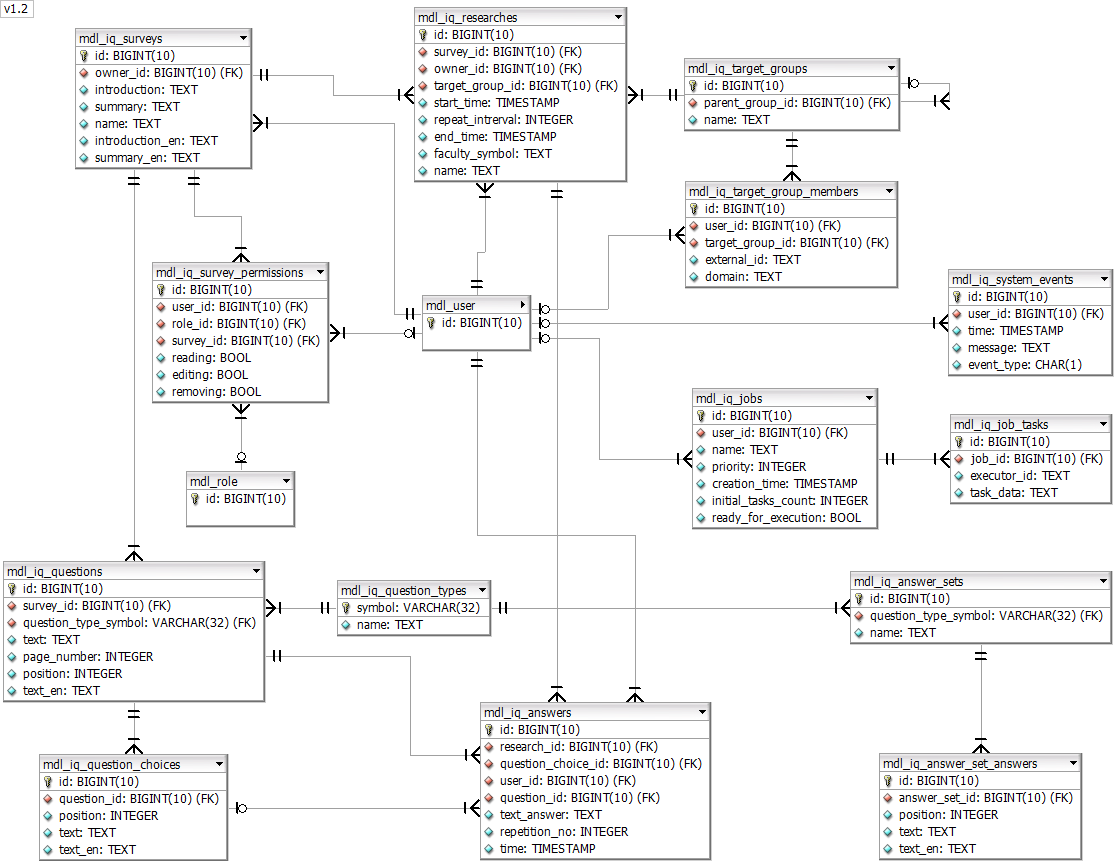
\includegraphics[height=\textheight, width=1.5\textwidth]{figures/iQuest_Database}
\caption{Diagram Bazy Danych}\label{rys:iQuest_DataBase}
\end{figure}
\end{landscape}